%
% File: chap02.tex
% Author: ta16969
% Description: !!!!!!!!!.
%
\let\textcircled=\pgftextcircled
\chapter{Artemis Design and Implementation}
\label{Artemis Design and Implementation}

\initial{T}his chapter introduces and explains the implementation of Artemis.After introducing the key features identifying the \textit{What?} and the \textit{Why?} aspects of Artemis it delves into the details of the three overriding design values used to inspire development i.e. OER, Captology (Web Credibility), Security and Accessibility.


\section{Development Tools and Languages}

Artemis has been developed using XAMPP-VM so as to use XAMP for Linux within the OS X environment, using the convienience of the OS X hypervisor to emulate a development environment that can be expected of industry standard production \cite{ApacheFriends.org}. Therefore Artemis has been predominantly written in PHP, served by Apache and uses MariaDB as it's SQL database. An alternative NoSQL stack was considered, specifically the MeteorJS full stack, however it was dismissed as being too niche and unsuitable for the OER modality of the tool; a more conventional SQL oriented stack is considered desirable for building a social network as evidenced by the experience of other social network developers \cite{Mei}.

Cross browser compatibility is outside of the scope of this project. However during development and evaluation the product has been used indiscriminately between Google Chrome, Mozilla Firefox (Developer Edition) and Safari. This approach helped target niche vendor specific issues, however it is stressed that complete cross compatibility is beyond the scope of the project and has not been explicitly attempted beyond the general good development practice of using multiple industry leading browsers.







\section{Stakeholder Assessment and Participation}

In an earier sub-section titled  \textit{Three Principle Stakeholders} it was determined that to enable a desirable pedagogy it would be prudent to investigate the primary stakeholders of a flexible pedagogy \cite{Gordon2014}; i.e. the UoB TEL team, CS course instructors and the student cohort are to be considered so as to ensure the successful development, deployment and adoption of the solution. Therefore the primary stakeholders were consulted and involved in the development of Artemis as follows (Please note that the following provide an overview of the of work carried out; specific references towards the work done will be made where relevant):
\begin{itemize}
    \item \textbf{TEL Team}: The TELED (Technology Enhanced Learning and Education Development)  department at the University of Bristol has a wide administrative and applied research mandate that broadly seems to straddles procurement, deployment, adoption, training and research associated with TEL solutions at the UoB \cite{UniversityofBristol}. An informal meeting was sought with the TEL team, which resulted in a valuable opportunity to personally discuss the project with the entire team who have a first hand experience of past, present and future TEL projects deployed at the UoB, their development criteria and a demonstrable experience in identifying what leads to failure as opposed to success within the context of TEL solutions deployed at the UoB. It is interesting to note that the TEL team cited lack of instructor adoption, as opposed to student's adopting a technology as equally important to the latter. Indeed the meeting also revealed a declining interest in the use of student forums, which may make a social network a desirable outcome of this project (as the former is viewed as a dated solution).
    
    \item \textbf{Teachers}: Feedback from UoB course instructors was sought informally; Primarily from Dr David Bernhard and Dr Ian Holyer. The TELED department had specificallh indicated that there was a lack of instructor interest in TEL solutions at the CS department and this was elaborated upon by the CS instructors interviewed. It was primarily cited that most TEL solutions were not adopted for either or both of the following reasons:
    \begin{itemize}
        \item Poor or unreliable functionality.
        \item Poor or faulty visual aesthetics.
    \end{itemize}
    
    The rationale for lack of adoption cited can be corroborated against the values of \textit{Web Credibility} and persuasive design, which are discussed in greater detail in a later section. The findings of the aforementioned are embedded in the GUI design and also used as the basis of evaluating Artemis and subsequently re factoring it. Instructor values were iterative incorporated by asking for their feedback throughout the life of the project.
    
    \item \textbf{Students}: Possibly the most important of the three stakeholders as the majority of the users are expected to be students. UoB CS conversion students and CS undergraduate students were asked for their opinions via a focus group session to generate ideas for possible features to be developed for Artemis; Which generally resulted in requests for a \textit{Facebook-StackOverflow} style social network as opposed to other mainstream social networks. Students were also asked to use the product and test it thoroughly as part of an open ended evaluation (although they were asked to complete a list of prescribed tasks and finish a questionnaire, they were strongly encouraged to use Artemis and explore it. Students were also encouraged to try and break or hack the code to the best of their ability, to see if any bugs could be found. The details of the evaluation form can be found in Appendix I. Users were actively encouraged to try and break or explore Artemis to see if any bugs or edge cases could be discovered. The evaluation was concluded with a questionnaire designed on Web Credibility principles (discussed later). Based on the bugs reported, student feedback and the results of the questionnaire, Artemis's code was re-factored to reflect the necessary changes and make it more relevant for user values.
\end{itemize}


\section{Persuasive Web Design}

At the core of rationale for embedding  learning models \& methodologies, pedagogy and social networks to ultimately develop a TEL solution is the presumption that the application will influence it's users. A TEL solution unable to persuade users in a desirable manner, due to either lack of adoption or otherwise inefficacy, is a solution that will fail or perform poorly; A fact outlined via preliminary informal discussions with the TEL team at the UoB.

The broad research area of \textit{captology}, by the Stanford Persuasive Technology Lab (STPL) covers the somewhat controversial study of  how computer and applications can be designed to change what people think and do \cite{Fogg2002a,Fogg2002,Fogg2001,Fogg1999}. Whilst extensive research of this area is deemed beyond the constraints of the project, some consideration is given to the constituent factors that improve user acceptance and/or influence; \textit{Web Credibility} and resultantly \textit{Web Application Security} and \textit{User Accessibility}.

It is proposed that by enhancing web credibility and application security, security the TEL solution can be designed in a manner that enhances user acceptance and adoption; Effectively not just making the TEL solution more effective in achieving it's intended purpose, but also avoiding a common cause of failure for TEL solutions implemented at the UoB i.e. lack of adoption of applications by relevant users.








\subsection{Web Credibility}

One aspect of making a \textit{persuasive} TEL solution, is by enhancing \textit{web credibility}. Web credibility within the context of designing this TEL solution refers to embedding best practice during web development, so as to influence a user's perspective of trustworthiness of the tool itself \cite{Fogg2001,Fogg2002} i.e. making the social network ultimately more persuasive and fit for purpose, by enhancing user perceptions of reliability and trustworthiness of the application \cite{Fogg2001} and effectively improving user acceptance.


In view of the project constraints, it is proposed that web credibility for the proposed web application can be achieved by adopting  the \textit{Stanford Guidelines for Web Credibility} \cite{Fogg2002a}. These guidelines are effectively a condensed and easy to follow framework for developing a Web Credible application based on the extensive research carried out by the STPL and associates; effectively aiding web developers to enhance web credibility based on findings of quantitative research as opposed to mere intuition \cite{Fogg2002a,Fogg2002,Fogg1999}.

These are listed as follows and briefly explained within the context of developing a web based social network and possible use cases that can be developed:

\begin{enumerate}
    \item \textbf{"Make it easy to verify the accuracy of the information on your site ?"} \cite{Fogg2002a}:
    
    The recommendation by STPL here is to allow for third party support via citations, references and source material \cite{Fogg2002a}. There are several ways that this can be embedded in the design of the proposed social network. Some proposed design features for the TEL solution that enhance this are :
    \begin{enumerate}
        
        \item Allow for annotation functionality to a web page via open source JavaScript libraries such as annotatorJS. The idea here is that it allows and encourages users to comment and add third party references to give assurance as to the source of information and it's quality.
        \item Allow for "likes". "Liking" a post on a social network and perhaps differentiating likes between the type of user e.g. a separate likes for users who are students and users who are instructors/experts, allows the content being portrayed by the social network to be verified or audited by experts and the community alike, from the view point of a user.
        \item A simple functionality is allowing for an encouraging URL's and relevant rich meta-data to be posted along with corresponding meta-data on the social network's user pages.
    
    \end{enumerate}
    
    \newpage
    \item \textbf{"Show that there's a real organization behind your site"} \cite{Fogg2002a}:
    
    This recommendation by the STPL can be satisfied by seeking explicit support from the UoB.  Initial introductory meetings with the UoB TEL team have been relatively, positive and it is tentatively believed that some form of association with the UoB will be inevitable if the tool is deployed, thus creating relevant user assurance.
    
    Furthermore deliverables such as a user and developer manuals have been proposed, so as to enhance this aspect of web credibility.
            
    \item \textbf{"Highlight the expertise in your organization and in the content and services you provide."} \cite{Fogg2002a}:
    
    To conform with this recommendation, it is considered that the salient features of the research based rationale for developing the TEL solution be shared on developer social networks such as GitHub along with it's source code, and be made accessible via the TEL solution as well for non-developers via a mission summary and a link to the project's GitHub page. i.e. user and developer relevant information is to be disseminated as part of this project's proposed deliverables. These shall be clearly accessible from the application's UI.
    
    \item \textbf{"Show that honest and trustworthy people stand behind your site"} \cite{Fogg2002a}:
    
    STPL recommends showing users that the people behind the web application are \textit{real} \cite{Fogg2002a}. This can be achieved in several ways:
    \begin{enumerate}
        \item Allowing for rich contextual data to be illustrated to the user when viewing other user's profiles i.e. users are able to determine that other profiles on the network either belong to fellow students or expert instructors.
        \item A separate page for biographical information of the developers as recommended by the STPL \cite{Fogg2002a}.
    \end{enumerate}
    
    \item \textbf{"Make it easy to contact you."} \cite{Fogg2002a}:
    It is proposed that this can be done by simply adding developer contact details for bug reports, suggested improvements and feedback via the social networks UI. Furthermore similar steps can be taken when disseminating developer and user manuals/related information.

    \item \textbf{"Design your site so it looks professional (or is appropriate for your purpose)"} \cite{Fogg2002a}:
    
    STPL recommends that this can be achieved by making evaluating the visual design of a web page, as users make quick evaluations based on visual design alone \cite{Fogg2002a}. It is proposed that this can be done by iteratively carrying out user acceptance tests i.e. by gaining feedback at regular intervals from fellow students and the research supervisor, about the aesthetic features of the TEL solution.

    \item \textbf{"Make your site easy to use"} \cite{Fogg2002a}:
    
    It is proposed that this can be done by simply seeking design inspiration from familiar social networks such as Facebook and Wikipedia, as users are likely to be familiar with the lay out and design of these sort of web applications\cite{Fogg2002a}.
    
    Furthermore user accessibility is considered in the following sections of this chapter.
    
    \item \textbf{"Update your site's content often (at least show it's been reviewed recently)."} \cite{Fogg2002a}:
    
    This should not be a problem within the context of a Web 2.0 application as the content is generated by users themselves and contributions from the developer are unlikely to be frequently required.
    
    \item \textbf{"Use restraint with any promotional content."} \cite{Fogg2002a}:
    
    As this is not a commercial venture, it is proposed that this can be avoided by banning the use of promotional ad content altogether during the development of the project.
    
    \item \textbf{"Avoid errors of all types, no matter how small they seem."} \cite{Fogg2002a}:
    
    Once again this can be sifted out during development via user acceptance testing and after deployment by allowing for active bug reports. Constant review of the web applications static content during development should mitigate this risk as well.
\end{enumerate}
\newpage


\section{Web Application Security}

With the transition of the world wide web from web-sites to web applications, i.e. the transition towards Web 2.0, a new host of security vulnerabilities moving away from traditional server side vulnerabilities towards new vectors such as client side have arisen \cite{Dayfdd2011}. Given the underlying importance of addressing common Web Application Security vulnerabilities \cite{Dayfdd2011} and it's negative impact on areas including but not limited to web credibility \cite{Fogg2002a,Fogg1999} that can affect the overall success and efficacy of the tool and even harm the users, this issue must be addressed.

\subsection{OWASP}

An extensive review of web application security is desirable but beyond the reasonable constraints of this project. Therefore  utilising the \textit{Open Web Application Security Project (OWASP) Top 10} \cite{OWASP2017} for identifying common or important design vulnerabilities and mitigating them will be used during development, as a viable alternative achievable within the constraints of the project.

The Open Web Application Security Project is an online community  and  a respected  not for profit organisation which creates free to use articles, methodologies, documentation, tools, and technologies towards the benefit of web application security \cite{OWASP}. The organisation  annually releases research that identifies and underlines mitigation strategies for the \textit{"Ten Most Critical Web Application Security Risks"}\cite{OWASP2017} identified threat agents within the scope of qualitative benchmarks i.e. possible attack vectors, the prevalence and detectability of security vulnerabilities, the technical implications and the commercial/business implications.

The rationale behind these qualitative benchmarks to assist the quantification and ranking of security risks,  is illustrated as via the help of the following diagram:

% A single figure
\begin{figure}[H]
	\centering
	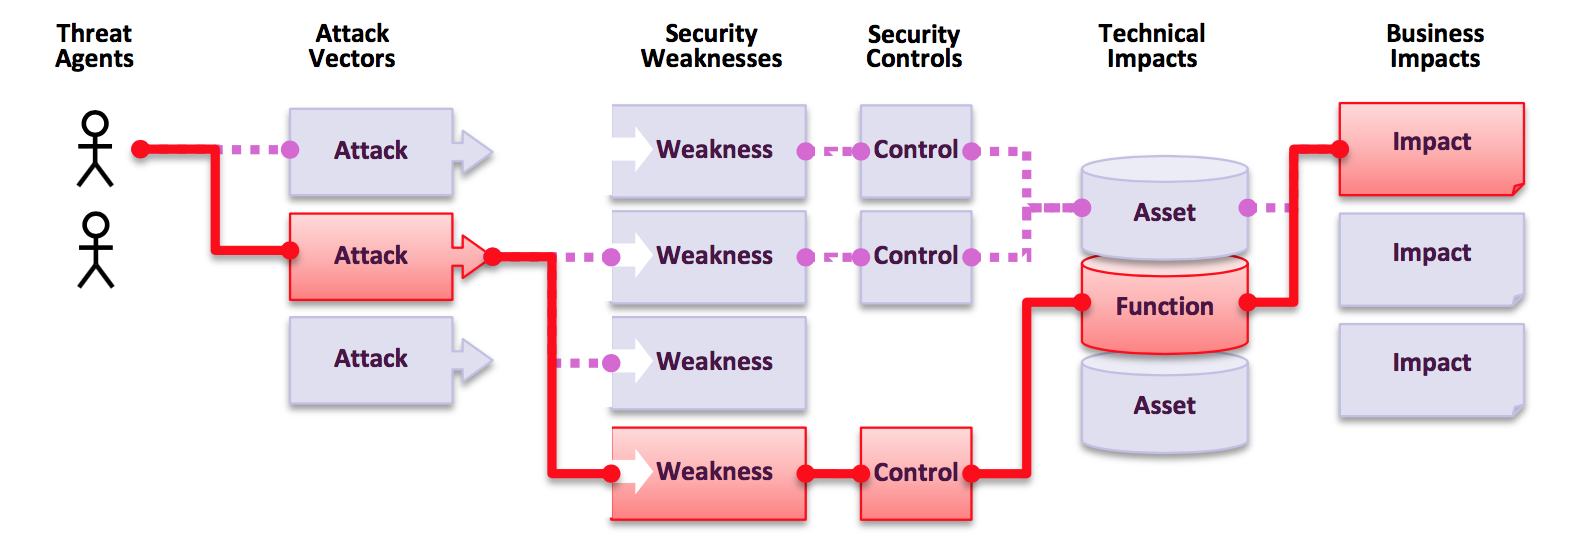
\includegraphics[scale=0.5]{figures/attack}
	\mycaption[Application Security - Consideration of Threat Agents]{Considerations of Threat Agents - . Figure reproduced from \cite{OWASP2017}.}
	\label{fig:Consideration of Threat Agents}
\end{figure}

The OWASP foundation reasons \cite{OWASP2017} that attackers or threat agents can exploit various modes of attack or \textit{attack vectors}, based on \textit{prevalence} and ease of \textit{detecting security weaknesses} (vulnerabilities) that can have a negative impact  within a generic technical or application specific commercial context \cite{OWASP2017}. Apart from application specific implications, the rest of these benchmarks can be classified based on the severity; which results in classification for the purpose of ranking the OWASP Top 10 vulnerabilities:

% A single figure
\begin{figure}[H]
	\centering
	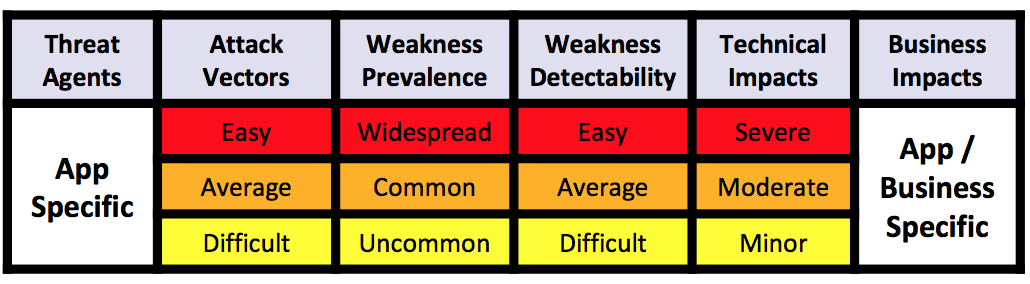
\includegraphics[scale=0.85]{figures/tabulation}
	\mycaption[OWASP Risk Rating Methodology]{OWASP Risk Rating Methodology - . Figure reproduced from \cite{OWASP2017}.}
	\label{fig:OWASP Risk Rating Methodology}
\end{figure}

Finally the risk rating methodology is used to compile an annual list of the most common, detectable and damaging security threats, along with mitigation strategies \cite{OWASP2017}. The proposed OWASP Top 10 for 2017, is effectively a mitigation strategy for this project that considers likelihood and impact. These are to be incorporated into the technical development of the TEL solution during development via consideration of the following (note there are various application and use specific mitigation strategies offered by OWASP and vendors, that will only be relevant when the actual product enters development. Predicting them in advance seems futile and therefore will be specifically explored during actual project development):

\begin{enumerate}
    \item \textbf{Injection}:
    
    Injection flaws, such as SQL and XML External Entity (XXE) injection may occur when untrusted data is sent to an interpreter as part of a query or command resulting in the execution of  unintended commands or accessing social/personal data without proper authorization \cite{OWASP2017}.

    \item \textbf{Broken Authentication and Session Management}:
    
    Authentication and/or session management functionality are often implemented incorrectly \cite{OWASP2017}. Effectively this could allow malicious attackers to compromise passwords, keys, or session tokens, and other flaws via assuming a victim's identity on the social network \cite{OWASP2017}.
    

    \item \textbf{Cross Site Scripting (XSS)}:
    
    XSS vulnerabilities include the inclusion of untrusted data in a new web page without proper validation or escaping, or updates an existing web page with user supplied data using a browser API that can create JavaScript. This allows the execution of malicious scripts in the victim browser \cite{OWASP2017}.
    
    \newpage
    
    \item \textbf{Broken Access Control}:
    
    Lack of restriction based on the authentication of users may result in  malicious access to unauthorized functionality and/or data, such as access to other user accounts, view sensitive files, modify other user's data and  changing access rights \cite{OWASP2017}. The organisation also provides a list of weak or redundant encryption keys and protocols, along with alternative modern ones that are more secure \cite{OWASP2017}.
    
    \item \textbf{Security Misconfiguration}:
    
    As per OWASP \cite{OWASP2017} recommendations good security requires having a secure configuration defined and deployed for the application, frameworks, application server, web server, database server etc. To do this secure settings should be defined, implemented, and maintained, as defaults are often insecure, a matter to be considered for the technical report. Additionally, software should be kept up to date\cite{OWASP2017}, therefore relevant notes will have to be made in the delevoper manuals disseminated on open source platforms.
    
    \item \textbf{Sensitive Data Exposure}:
    
    Particularly relevant to web applications such as this project which collect social data, APIs do not properly protect sensitive data, which attacker may misuse. OWASP recommends modern encryption strategies to mitigate the risk of security breaches, anticipated or otherwise, e.g. using strong purpose built algorithms and simply dropping data from databases that regularly, that is not useful for commercial/app specific purposes \cite{OWASP2017}.
    
    \item \textbf{Insufficient Attack Protection}:
    
    This refers to app vulnerabilities such as APIs which lack the basic ability to detect, prevent, and respond to both manual and automated attacks \cite{OWASP2017}. It bears noting that this area covers proactive and reactive mitigation strategies well beyond the scope of the project, despite considerations that may be given to blocking automated and manual malicious attacks during the course of development.
    
    \item \textbf{Cross Site Request Forgery (CSRF)}:
    
    A CSRF attack forces a logged-on victim's browser to send a forged HTTP request, including the victim’s session cookie and any other automatically included authentication information, to a vulnerable web application \cite{OWASP2017}. OWASP recommends using pre-existing CSRF defenses available within most modern frameworks.
    
    \item \textbf{Using Components with Known Vulnerabilities}:
    
    Components, such as libraries, frameworks, and other software modules, run with the same privileges as the application and if a vulnerable component is exploited,  an attack can facilitate  a plethora of malicious activities \cite{OWASP2017}.
    
    Most mitigation strategies in this area are usually reactive (beyond researching components before using them), thus deemed outside of the constraints of this report.
    
    \item \textbf{Underprotected API's}:
    
    "Modern applications often involve rich client applications and APIs, such as JavaScript in the browser and mobile apps, that connect to an API of some kind (SOAP/XML, REST/JSON, RPC, GWT, etc.). These APIs are often unprotected and contain numerous vulnerabilities" \cite{OWASP2017}.
    
    This is a relatively new area of vulnerability being studied for the purpose of mitigation strategies by OWASP \cite{OWASP2017}; generally beyond the reasonable constraints of this project. A proposed mitigation strategy available here, is to perhaps consider expert advise from security experts and practitioners of relevant client applications.
    
\end{enumerate}




\section{Accessibility}

Making a tool user accessible is an important consideration when deploying a TEL solution, within the context of UoB students as per preliminary meetings with the UoB TEL team. Furthermore user accessibility enhances both the persuasiveness of the TEL solution and it's web credibility. However it is recognised that accessibility issues can cover a wide range of impairments within the broad blanket categories such as audio, visual and mobility impairments \cite{Mills2015}. An extensive accessibility review for this project, is beyond it's reasonable constraints as mitigation for every possible impairment is impossible to implement, and is usually reactive in nature as per the UoB TEL team.

It is proposed that by following best practice on at least visual impairment (likely the most important of the three within the context of this project) as recommended by the MDN's (Mozilla Developers Network) guidelines \cite{Mills2015,Mills2016} on accessibility and W3C's (World Wide Web Consortium) Web Accessibility Initiative (WAI) for developers \cite{W3C}, a satisfactory level of accessibility can be embedded in the design of the tool.

\subsection{Accessible HTML, CSS and JavaScript}

HTML, CSS and JavaScript are basic building blocks in most web applications such as the proposed social network and by following specific best practice at the time of development to enhance accessible device interaction, the need for using tools such as WAI-ARIA can be reduced \cite{W3C,OWASP,Mills2015,Mills2016}. As opposed to CSS and JavaScript, HTML is cited as having the greatest implications (negative and positive)  within the context of interaction with relevant accessibly devices e.g. screen readers \cite{Mills,Mills2017} and ultimately an impact on user accessibility.  It is highlighted that the nuances of enhancing accessibility are different for all of the aforementioned technologies; however they are condensed in the interest of brevity into overlapping points of best practice as follows:


\begin{enumerate}
    \item \textbf{Semantically Sensible Code}:
    
    This refers to the use of the correct semantic language elements for the correct purpose e.g. using breaks, paragraphs and specific HTML tags for intended purposes only \cite{Mills,Mills2017} to create a semantically sensible layout of data, so that screen readers which are developed with certain expectations/assumptions can operate correctly.
    
    Within the context of HTML this refers to using semantic HTML otherwise referred to as POSH (plain old semantic html) HTML \cite{Mills2017} and for CSS and JavaScript (JS) using semantically sensible code \cite{Mills}. The rationale for using semantically similar and plain code is that it is more likely to conform to client-device expectations and result in a smoother user interaction experience via accessibility devices such as screen readers \cite{Mills2017,Mills}.
    
    \item \textbf{Unobtrusive and Flexible Code}:
    
    Client side devices such as screen readers effectively take control of the code in a web application, which for the sake of accessibility as well as technical flexibility should be accepted during development e.g. users may override CSS to use custom style sheets to read content more easily \cite{Mills}. Beyond merely accepting the possibility of overriding control, CSS and JS in particular should be developed to make this easier for screen readers and accessibility devices \cite{Mills,Mills2017,Sukardi2016} i.e. writing flexible code that is unobtrusive towards user devices e.g. Developing client-side form validation, which alerts users to problems with their form entries quickly,as opposed to server-side form validation which would take longer and cause problems or confusion from the perspective of a visually impaired user using a screen reader. 
    
    Assuming the usage of POSH HTML, this requirement extends to writing more flexible and unobtrusive CSS and JS. As such it would be impractical to envision and identify every possible use case, however it suffices to say that writing flexible and unobtrusive code is not always possible given the complexity of modern UI's that require unsemantic HTML5 features and dynamic content generating JS, indicative that alternative tools will be necessary as well \cite{Mills,Sukardi2016}, discussed in the next section.


    \item \textbf{Colour Contrast}:
    
    
    MDN guidelines recommend accommodating  colour blind accessibility via the use of colour contrast checkers during web development \cite{Mills}. This would can allow for iterative testing during the development process, to assess whether the site is readable from the perspective of a colour blind person and more than merely aesthetically pleasing CSS. It is also recommended to use non-colour alternatives  to aid document semantics, along with colour based semantic aids \cite{Mills} e.g. altering the fonts along with font colour to highlight text, effectively making the highlighted text visible to colour blind users. By using non-visual cues, people impaired by colour blindness are more easily able to detect patterns and text.
    
\end{enumerate}

\subsection{WAI-ARIA (Web Accessibility Initiative - Accessible Rich Internet Applications)}

Semantically well formed HTML, CSS and JS is recommended as a first port of call for making UI's accessible \cite{Sukardi2016}. However as discussed earlier, given the complexity of a social network's UI which is almost certainly going to use  dynamic JS updated content, if not unsemantic HTML5 features an alternative tool is necessary \cite{Sukardi2016}.


In such instances WAI-ARIA  \cite{W3C,February2016a,Sukardi2016} seem to be the viable alternative for this project. WAI is a specification written by the W3C \cite{W3C,Sukardi2016} which adds additional semantic attributes to a web application's HTML. ARIA is a technology that can help  by adding in further semantics that browsers and assistive technologies can recognize and use, benefiting the user experience of accessibility challenged clients \cite{W3C,Sukardi2016}. 

ARIA technology is supported by W3C via the WAI \cite{W3C,February2016a}, has good global browser support \cite{Sukardi2016} and is supported by most major screen reader used in the area \cite{Sukardi2016}. ARIA has many features and resultant use cases, some of which might not be relevant or feasible for this project \cite{February2016a}.Within the context of this specific project WAI-ARIA's many tools can be used for the following :

\begin{enumerate}
    \item Semantic Enhancement: WAI-ARIA can enhance the semantic attributes of HTML for this project. Alternatively, it can be used to replicate HTML semantics where none are possible to implement via HTML itself.
    \item Dynamic content updates: The use of dynamically updated content via JS is unavoidable for this project, which unfortunately screen readers tend to have difficulty with \cite{Sukardi2016,Mills}. ARIA utilises technology that can inform screen readers of content updates to the screen and effectively any new content generated in a social  network \cite{Sukardi2016}.
    \item Assisting Non-Semantic Complex UI's and Control: UI's or menus that utilise nested HTML div tags, along with JS and CSS can benefit from advanced control features, however interpreting them from the perspective of a screen reader device can be very difficult. ARIA provides functions and tools, capable of providing clues to a screen reader as to how to go about navigating a complex UI.
\end{enumerate}

Before concluding this chapter it must be reiterated that accessibility is a desirable feature for this project. However an extensive  review to make the web application accessible for all eventualities is deemed unfeasible in light of the project constraints. Therefore the whilst certain accessibility mitigation strategies such as semantic,flexible and unobtrusive programming for HTML,CSS and JS will be incorporated into design, evaluation via screen readers and embedding ARIA enhanced semantics where necessary will  implemented as an optional deliverable/extension, if the project constraints allow it.


